% \subsection{Dataset di partenza}
Il dataset è stato realizzato analizzando i dati corrispondenti ai risultati delle partite di Premier League
dalla stagione 2008/2009 alla stagione 2018/2019.
Successivamente, il lavoro è stato svolto con un dataset caratterizzato da 4180 righe x 78 colonne, 
36 squadre e 40 features, poi utilizzate per la manipolazione ed estrazione di 38 features.

Ciascuna partita è caratterizzata dal \textit{country id, league id, season, stage, date, match api id,
home team id, away team id, home team goal, away team goal, home player X positions,
away player X positions, home player Y positions, away player Y positions, home player ids,
away player ids} e le quote delle varie scommesse \textit{(B365A, B365D, B365H, BSA, BSD, BSH, BWA, BWD, . . . .)}

Mentre per ogni squadra si ha il \textit{team id, team name, FIFA id, FIFA data 
and FIFA statistics} (che includono build up play speed, build up play dribbling, etc.).
Poiché quest'ultimi dati erano inconsistenti e senza alcuni valori, 
sono stati utilizzati per definire il ranking ELO (andamento complessivo di una squadra) e la correlazione. 

\begin{figure}[h]
        \centering
        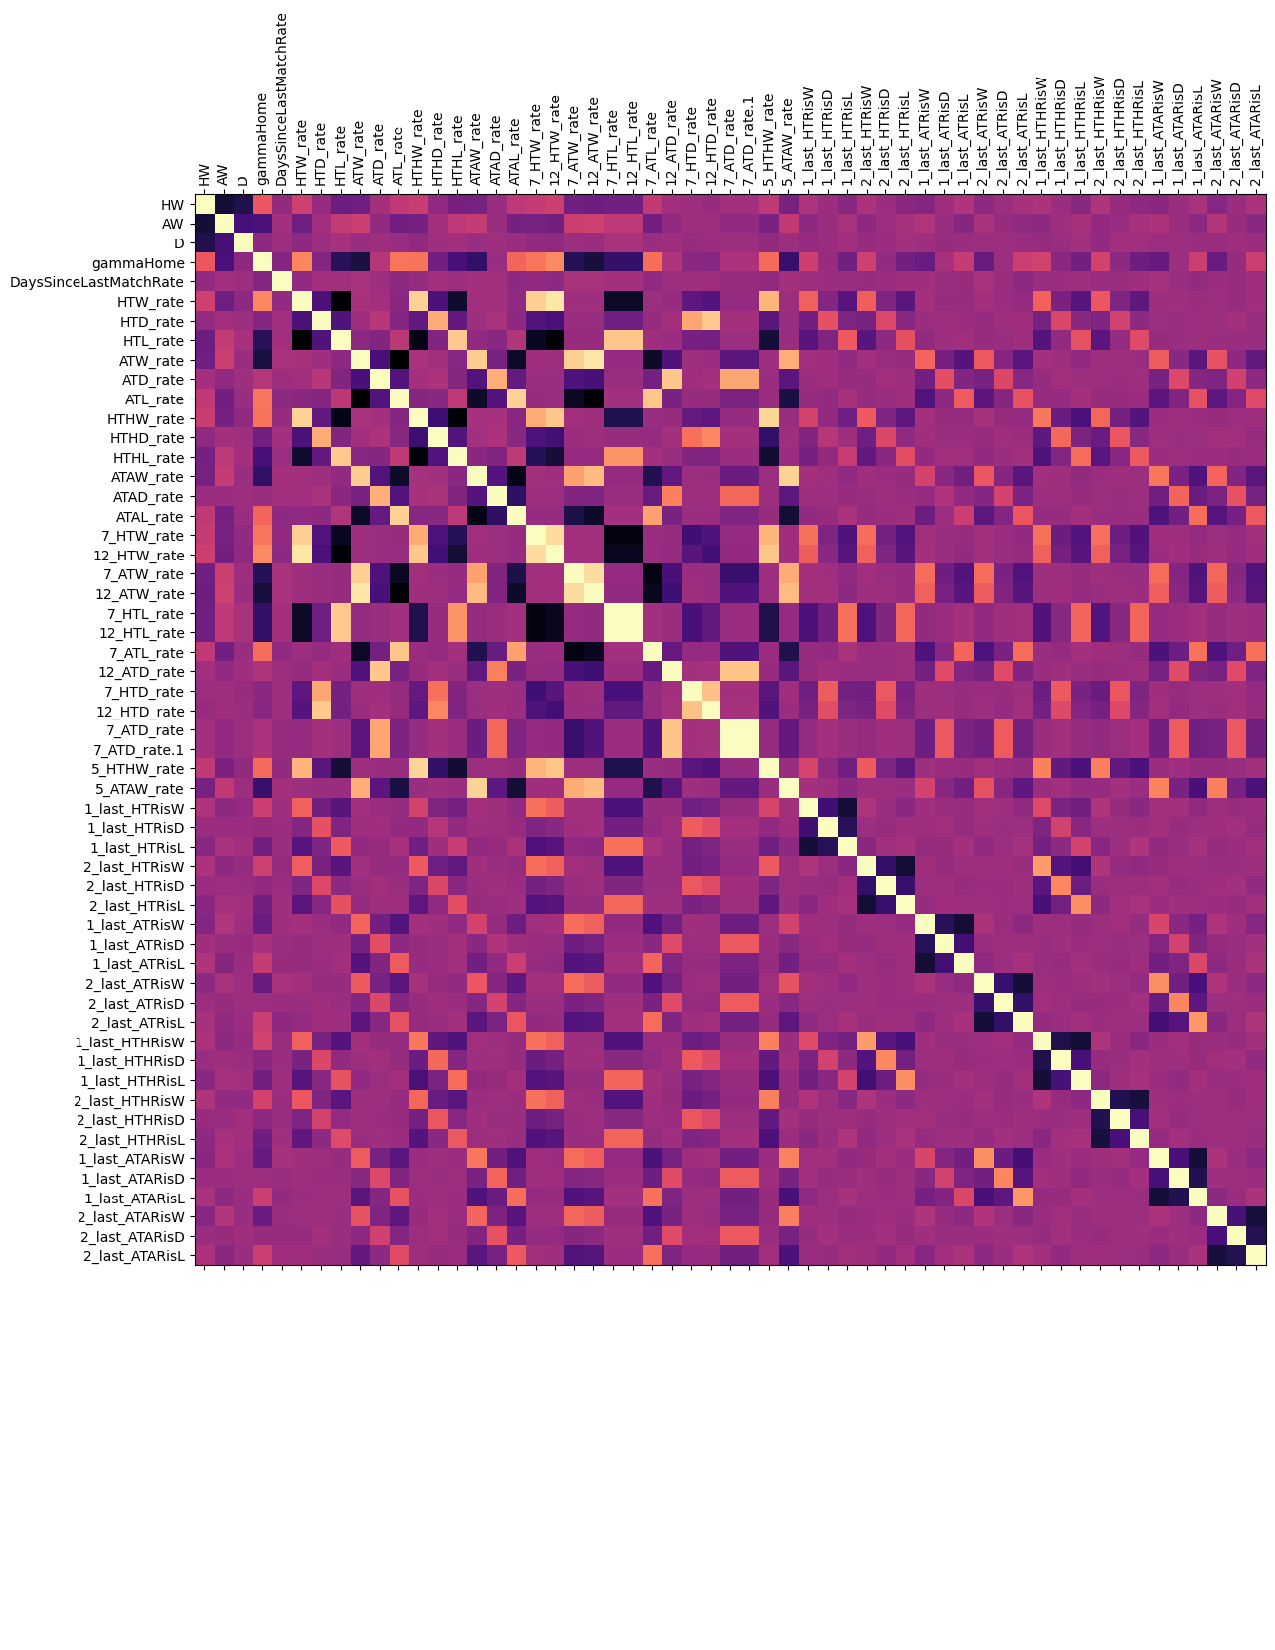
\includegraphics[scale=0.5]{tesina/img/corr_feat.pdf}
        \caption{Correlazioni tra tutte le features (regioni più chiare corrispondono a valori di correlazione maggiori)}
\end{figure}

\newpage
A conclusione del progetto, sono state utilizzate 24 features: 
\begin{table}[!h]
\resizebox{\textwidth}{!}{%
    \centering
    \begin{tabular}{|c|c||c|c|}
    \hline
         Home team & HomeTeam & Last 7 home team win rate & 7\_HTW\_rate\\
         \hline
         Away team & AwayTeam & Last 7 home team lose rate & 7\_HTL\_rate \\
         \hline
         Home team ELO score & HTeamEloScore & Last 7 home team draw rate & 7\_HTD\_rate \\
         \hline
         Away team ELO score & ATeamEloScore & Last 7 away team win rate & 7\_ATW\_rate \\
         \hline
         Home team days since last match & HTdaysSinceLastMatch & Last 7 away team lose rate & 7\_ATL\_rate\\
         \hline
         Away team days since last match & ATdaysSinceLastMatch & Last 7 away team draw rate & 7\_ATD\_rate \\
         \hline
         Home team win rate & HTW\_rate & Last 12 home team win rate & 12\_HTW\_rate \\
         \hline
         Away team win rate & ATW\_rate & Last 12 home team lose rate & 12\_HTL\_rate \\
         \hline
         Home team draw rate & HTD\_rate & Last 12 home team draw rate & 12\_HTD\_rate \\
         \hline
         Away team draw rate & ATD\_rate & Last 12 away team win rate & 12\_ATW\_rate \\
         \hline
         Last 5 home team home win & 5\_HTHW\_rate & Last 12 away team lose rate & 12\_ATL\_rate\\
         \hline
         Last 5 away team away win & 5\_ATAW\_rate & Last 12 away team draw rate & 12\_ATD\_rate \\
         \hline
    \end{tabular}}
    \caption{Features selezionate e la loro abbreviazione}
    \label{tab:featAbbr}
\end{table}

\begin{figure}[h]
    \centering
    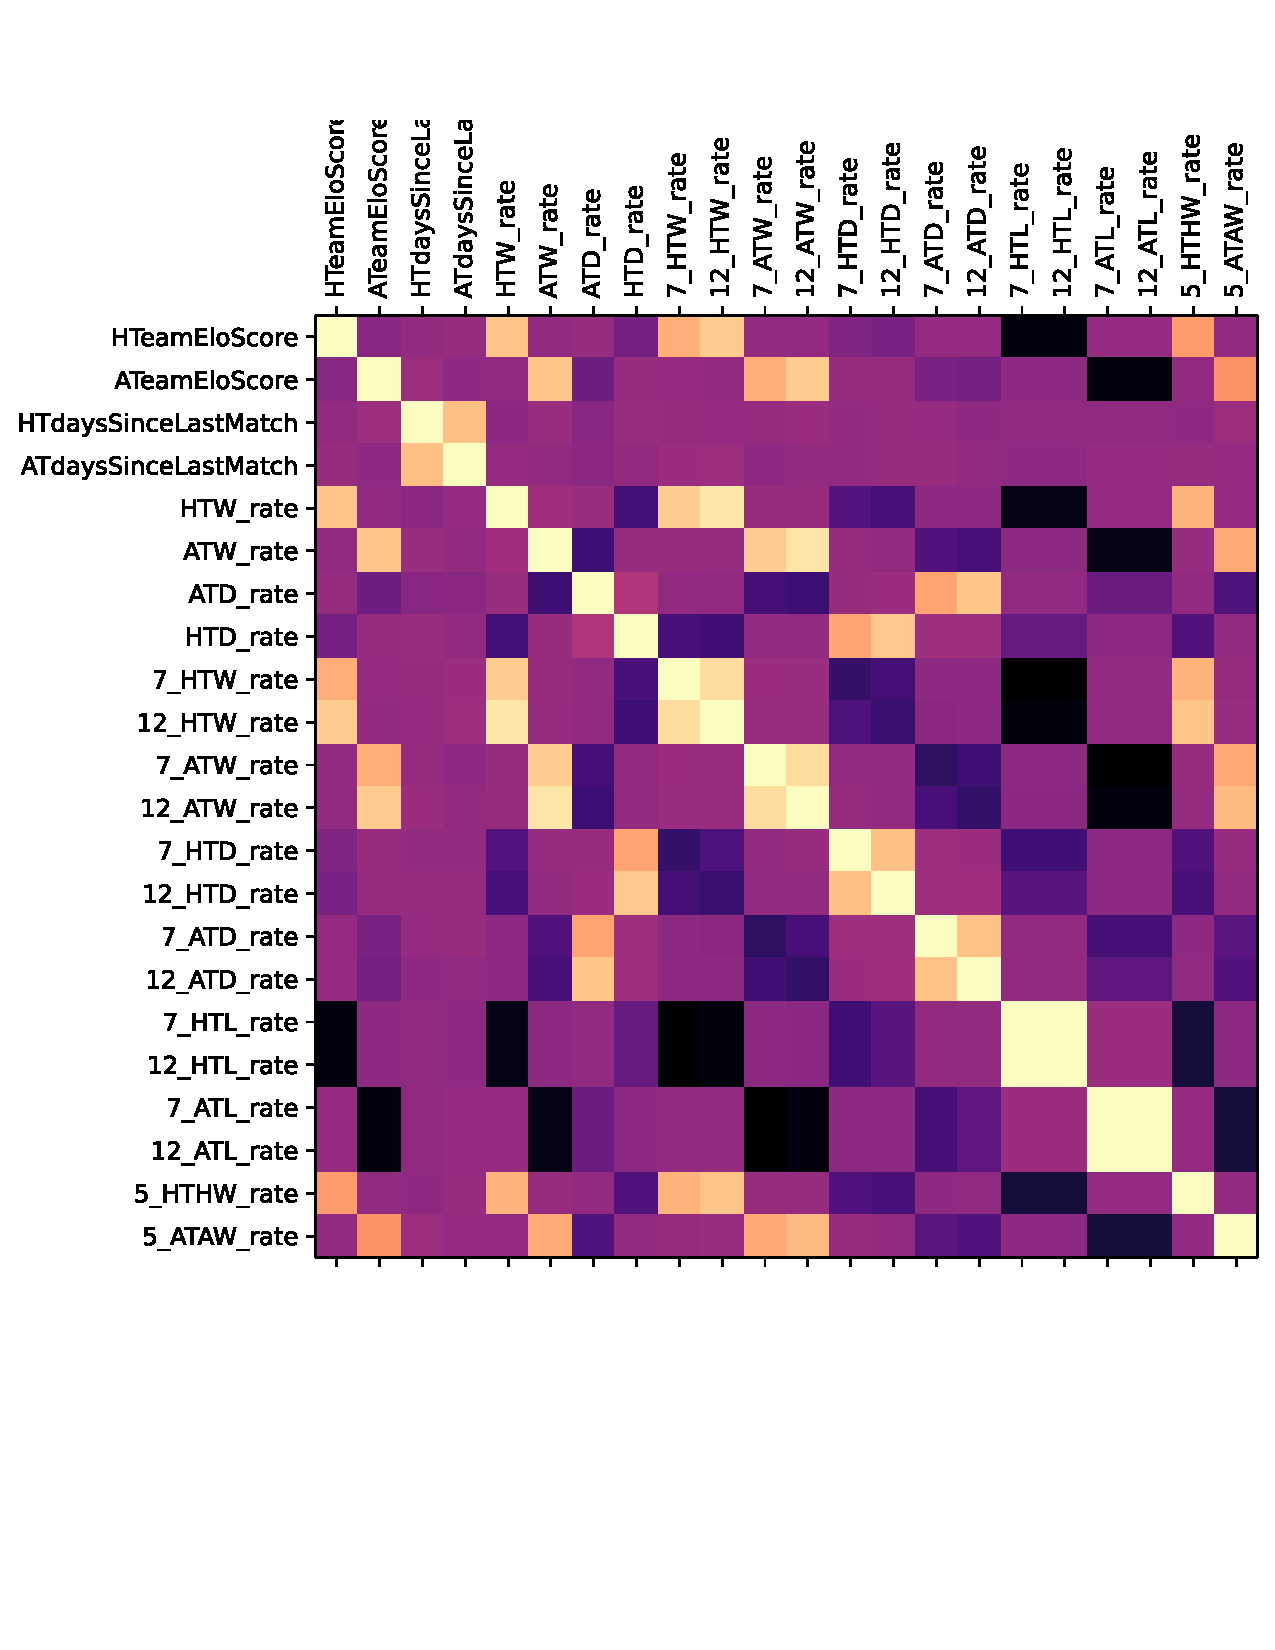
\includegraphics[scale=0.4]{tesina/img/corr_sel_feat.pdf}
    \caption{Correlazione tra le features selezionate (regioni più chiare corrispondono a valori di correlazione maggiori)}
    \label{fig:lstmColFeatures}
\end{figure}